%%%%%%%%%%%%%%%%%%%%%%%%%%%%%%%%%
%Preamble
%%%%%%%%%%%%%%%%%%%%%%%%%%%%%%%%%

\PassOptionsToPackage{usenames, dvipsnames, table}{xcolor}

\documentclass[aspectratio=169]{beamer}
\usetheme{Boadilla}

%Make beamer number figures, because it doesn't by default
\setbeamertemplate{caption}[numbered]

\usepackage[english]{babel}
\usepackage[ruled, vlined]{algorithm2e}

\usepackage{amsfonts}
\usepackage{setspace, graphicx, epstopdf, amsmath}
%Do not use enumitem because this interferes with beamer drawing bullet points
\usepackage{marginnote, datetime, url, subfigure}

%Bibliography Stuff
%Use natbib even though it's old because it's compliant with journal styles
%Actual bibliography style etc are specified where you actually want it
\usepackage{natbib}


%Fluff
\linespread{1.3}

%Neural Network Packages
\usepackage{neuralnetwork}
\usepackage{xpatch}
\makeatletter
% \linklayers have \nn@lastnode instead of \lastnode,
% patch it to replace the former with the latter, and similar for thisnode
\xpatchcmd{\linklayers}{\nn@lastnode}{\lastnode}{}{}
\xpatchcmd{\linklayers}{\nn@thisnode}{\thisnode}{}{}
\makeatother

%Regression Tree
\usepackage{tikz,forest}
\usetikzlibrary{arrows.meta}

\forestset{
	.style={
		for tree={
			base=bottom,
			child anchor=north,
			align=center,
			s sep+=1cm,
			straight edge/.style={
				edge path={\noexpand\path[\forestoption{edge},thick,-{Latex}] 
					(!u.parent anchor) -- (.child anchor);}
			},
			if n children={0}
			{tier=word, draw, thick, rectangle}
			{draw, diamond, thick, aspect=2},
			if n=1{%
				edge path={\noexpand\path[\forestoption{edge},thick,-{Latex}] 
					(!u.parent anchor) -| (.child anchor) node[pos=.2, above] {Y};}
			}{
				edge path={\noexpand\path[\forestoption{edge},thick,-{Latex}] 
					(!u.parent anchor) -| (.child anchor) node[pos=.2, above] {N};}
			}
		}
	}
}

%%TODONOTE commands
\usepackage[colorinlistoftodos]{todonotes}
\newcommand{\smalltodo}[2][] {\todo[caption={#2}, size=\scriptsize,%
	fancyline,#1]{\begin{spacing}{.5}#2\end{spacing}}}
\newcommand{\rhs}[2][]{\smalltodo[color=green!30,#1]{{\bf RS:} #2}}
%%

%Graphs
\usepackage{tikz}
\usepackage{pgfplots}

\usepackage[export]{adjustbox}

%Coloured Tables


%%%%%%%%%%%%%%%%%%%%%%%%%%%%%%
%%Title and other fluff, just before document start
%%%%%%%%%%%%%%%%%%%%%%%%%%%%%%

%Hyperref apparently is a big package and causes a lot of issues, so it's recommended to load this last

\usepackage{hyperref}

%Gets rid of the neon green boxes around boxes

\usepackage[]{xcolor}

\graphicspath{{../Results/}}

\hypersetup{
	colorlinks,
	linkcolor = {red!50!black},
	citecolor = {blue!50!black},
	urlcolor = {blue!80!black}
}

\title{Evaluation of Machine Learning in Finance}

\author{Ze Yu Zhong 
	\\ Supervisor: David Frazier}

\institute{Monash University}

\date{}

\begin{document}
	
\begin{frame}[plain]
    \maketitle
\end{frame}

%%%%%%%%%%%%%%%%%%%%%%%%%%%%%%%%%%%%%%%%%%%%%%%%%%%%
\section{Introduction}
%%%%%%%%%%%%%%%%%%%%%%%%%%%%%%%%%%%%%%%%%%%%%%%%%%%%

%%%%%%%%%%%%%%%%%%%%%%%%%%%%%%%%%%%%%%%%%%%%%%%%%%%%%
%%Intereave literature review throughout this section
%%%%%%%%%%%%%%%%%%%%%%%%%%%%%%%%%%%%%%%%%%%%%%%%%%%%%

\begin{frame}
\frametitle{Main Motivation}
To evaluate the application of machine learning to the problems of \textbf{prediction} and \textbf{causal inference} in empirical finance.
\end{frame}

\begin{frame}
\frametitle{Motivation}
Empirical finance is typically concerned with two main goals:
\begin{itemize}
	\item \textbf{Prediction} accuracy
	\item \textbf{Causal} inference
\end{itemize}
\end{frame}

\begin{frame}
\frametitle{Motivation}
These goals are very difficult, especially for traditional regression!

The underlying data generating process for financial data is unknown - returns are estimated by \textit{risk factors}, defined by \cite{harvey__2016} as a collection of regressors that can proxy for underlying risk factors

Factors are often unsuitable for regression:
\begin{itemize}
	\item Persistent
	\item Cross-sectionally correlated (multicollinearity)
	\item Non-stationary
	\item Pre-known or sampled at a lower frequency, exhibiting low time series variation
\end{itemize}
\end{frame}

\begin{frame}
\frametitle{Motivation}
Consequences when included in traditional regression well documented:
\begin{itemize}
	\item Biased t-stats
	\item High variance for coefficient estimates
	\item Unstable coefficient estimates
\end{itemize}
These can adversely affect statistical inference. 

The estimated coefficients, due to being imprecise, will also result in poor out of sample prediction, which are a function of coefficients. This is particularly so if the multicollinearity between regressors changes over time, which is likely in financial data
\end{frame}

\begin{frame}
\frametitle{Background - Dividend Ratio Example}
\begin{itemize}

\item Included due to good in sample performance in the 1990s \citep{goyal_predicting_2003}

\item \textit{Persistent} (\cite{goetzmann_testing_1993}, \cite{ang_stock_2006})

	\begin{itemize}
	\item Correlated with lagged dependent variables on the right hand side of the regression equation. 
	
	\item Violates assumptions of independent regressors of OLS: t stats are biased upwards due to autocorrelated errors
	
	\item GMM and NW errors corrections are also biased, \citep{goetzmann_testing_1993}
	\end{itemize}

\item Not robust and have poor out of sample performance since 2000s (\cite{goyal_predicting_2003}, \cite{lettau_consumption_2001}, \cite{schwert_anomalies_2003})
\end{itemize}
\end{frame}

\begin{frame}
\frametitle{Dividend Ratio Example}
\begin{itemize}
\item Factors such as dividend ratios, earnings price ratio, interest and inflation etc. were ``widely accepted" to be able to predict excess returns, \citep{lettau_consumption_2001}

\item \cite{welch_comprehensive_2008} conclude that not a single variable had any statistical forecasting power, and the significance values of some factors change with the choice of sample periods.
\end{itemize}
\end{frame}

\begin{frame}
\frametitle{Background}
\begin{itemize}
\item More factors produced by literature: currently over 600 documented \citep{harvey_census_2019}
\begin{itemize}
	\item False discovery problem, \citep{harvey__2016}
	
	\item Factors are cross sectionally correlated - inefficient covariances, factors may be subsumed within others, \citep{feng_taming_2019}
	
	\item Number of factors may be more than sample size, making regression impossible
\end{itemize}
\end{itemize}
\end{frame}

%%%%%%%%%%%%%%%%%%%%%%%%%%%%%%%%%%%%%%%%%%%%%%%%%%%%
\section{Why apply Machine Learning in Finance?}
%%%%%%%%%%%%%%%%%%%%%%%%%%%%%%%%%%%%%%%%%%%%%%%%%%%%

%%%%%%%%%%%%%%%%
%Interweave Literature review throughout this section
%%%%%%%%%%%%%%%%

\begin{frame}
\frametitle{Why apply Machine Learning in Finance?}

Machine learning methods have been used within the literature and appear to be well suited \textbf{as means of managing this factor explosion}:
\begin{itemize}
	\item Mlexible than traditional regression models, which make strong functional form assumptions and are sensitive to outliers, \citep{freyberger_dissecting_2017}
	\item Explicit ``regularization" methods for guarding against overfitting
	\item Better equipped to deal with high dimensionality
\end{itemize}
\end{frame}

\begin{frame}
\frametitle{Applications in the Literature}
Causal Analysis:
\begin{itemize}
	\item \cite{kozak_shrinking_2017}, \cite{rapach_forecasting_2013}, \cite{freyberger_dissecting_2017}, and others apply shrinkage and selection methods to assist with factor selection
\end{itemize}
Prediction Performance:
\begin{itemize}
	\item \cite{gu_empirical_2018}, \cite{feng_deep_2018}, construct machine learning portfolios that historically outperform traditional portfolios in terms of prediction error and predictive $R^2$
	\item Attribute their success to machine learning's ability to find non-linear interactions
\end{itemize}
\end{frame}

\begin{frame}
\frametitle{Motivations}
However, little work has been done on how machine learning actually recognises and deals with the challenges in financial data. 

Machine learning is mainly suited for specific contexts:
\begin{itemize}
	\item Often assume i.i.d., (\cite{murphy_quantifying_2010})
	\item Often require large amounts of data
	\item Struggle with state dependence, (\cite{bengio_learning_1994})
	\item Little interpretability in regressors - not too concerned with causal analysis
\end{itemize}
\end{frame}

\begin{frame}
\frametitle{Methodology Issues}
\begin{itemize}
	\item \cite{feng_deep_2018} \textbf{cross validates} their training set
	\item \cite{gu_empirical_2018} only use data up until the 1970s to produce predictions in the last 30 years
	\item \cite{gu_empirical_2018}'s models do not have consistent importance metrics - only their tree based methods recognise dividend yield as important
\end{itemize}
\end{frame}

\begin{frame}
\frametitle{Motivations}
Can machine learning assist with returns \textbf{prediction} and \textbf{causal} inference?
\begin{itemize}
	\item Persistent Regressors?
	\item Identify true factors from a high dimensional, cross sectionally correlated panel?
	\item Is regularization enough to handle non-robustness?
	\item Are their conclusions consistent?
	\item Do they perform better than traditional methods?
\end{itemize}
\end{frame}

\begin{frame}
\frametitle{Motivations}
We explored this via two studies, focusing on the prediction performance and factor selection performance of some common machine learning models:

Simulation study
\begin{itemize}
	\item Explicitly explore how machine learning performs in controlled environments
\end{itemize}

Empirical study
\begin{itemize}
	\item Validate our results
	\item Contrast them with literature
\end{itemize}
\end{frame}

%%%%%%%%%%%%%%%%%%%%%%%%%%%%%%%%%%%%%%%%%%%%%%%%%%%%
\section{Model Specification}
%%%%%%%%%%%%%%%%%%%%%%%%%%%%%%%%%%%%%%%%%%%%%%%%%%%%

\begin{frame}
\frametitle{Model Specification}
Returns are modelled as an additive error model
\begin{equation}
	r_{i, t+1} = E(r_{i, t+1} | \mathcal{F}_t) + \epsilon_{i, t+1}
\end{equation}
		
where 
\begin{equation}
	E(r_{i, t+1} | \mathcal{F}_t) = g^*(z_{i,t})
\end{equation}
		
Stocks are indexed as $i = 1, \dots, N$ and months by $t = 1, \dots, T$. 

$g^*(z_{i,t})$ represents the model approximation using the $P$ dimensional predictor set $z_{i,t}$. 
\end{frame}

%%%%%%%%%%%%%%%%%%%%%%%%%%%%%%%%%%%%%%%%%%%%%%%%%%%%
\section{Methodology}
%%%%%%%%%%%%%%%%%%%%%%%%%%%%%%%%%%%%%%%%%%%%%%%%%%%%

\begin{frame}
\frametitle{Overview}
Machine Learning Methodology consists of 3 overall components:
\begin{itemize}
	\item Sample Splitting
	\item Loss Function(s)
	\item Models/Algorithms considered
\end{itemize}

Overall methodology folloiws that of \cite{gu_empirical_2018}
\end{frame}

%%%%%%%%%%%%%%%%%%%%%%%%%%%%%%%%%%%%%%%%%%
%Sample Splitting
%%%%%%%%%%%%%%%%%%%%%%%%%%%%%%%%%%%%%%%%%%

\begin{frame}
\frametitle{Sample Splitting - Expanding Window Scheme}
\begin{figure}
	\begin{center}
		\begin{tabular}{|c|p{0.40cm}p{0.40cm}p{0.40cm}p{0.40cm}p{0.40cm}p{0.40cm}p{0.40cm}p{0.40cm}p{0.40cm}p{0.40cm}p{0.40cm}p{0.40cm}p{0.40cm}p{0.40cm}p{0.40cm}|}
			\hline
			Set No. &&&&&&&&&&&&&&& \\
			\hline
			%%%%%%%%
			3 & \cellcolor{cyan} & \cellcolor{cyan} & \cellcolor{cyan} & \cellcolor{cyan} & \cellcolor{cyan} & \cellcolor{cyan} & \cellcolor{cyan} & \cellcolor{cyan} & \cellcolor{cyan} &
			\cellcolor{pink} & \cellcolor{pink} & \cellcolor{pink} & \cellcolor{pink} & \cellcolor{pink} & 	
			\cellcolor{olive} \\
			%%%%%%%%
			2 & \cellcolor{cyan} & \cellcolor{cyan} & \cellcolor{cyan} & \cellcolor{cyan} & \cellcolor{cyan} & \cellcolor{cyan} & \cellcolor{cyan} & \cellcolor{cyan} &
			\cellcolor{pink} & \cellcolor{pink} & \cellcolor{pink} & \cellcolor{pink} & \cellcolor{pink} & 	
			\cellcolor{olive} & NA  \\
			%%%%%%%%
			1 & \cellcolor{cyan} & \cellcolor{cyan} & \cellcolor{cyan} & \cellcolor{cyan} & \cellcolor{cyan} & \cellcolor{cyan} & \cellcolor{cyan} &
			\cellcolor{pink} & \cellcolor{pink} & \cellcolor{pink} & \cellcolor{pink} & \cellcolor{pink} & 	
			\cellcolor{olive} & NA & NA \\
			\hline
			Year & 1 & 2 & 3 & 4 & 5 & 6 & 7 & 8 & 9 & 10 & 11 & 12 & 13 & 14 & 15\\
			\hline
		\end{tabular}
		\medskip
		\begin{tabular}{|c|p{0.40cm}|}
			\hline
			Training & \cellcolor{cyan} \\
			\hline
			Validation & \cellcolor{pink} \\
			\hline
			Test & \cellcolor{olive} \\
			\hline
		\end{tabular}
	\end{center}
	\caption{Sample Splitting Procedure}
	\label{sample_split_diag}
\end{figure}
\end{frame}

%%%%%%%%%%%%%%%%%%%%%%%%%%%%%%%%%%%%%%%%%%
%Loss Functions
%%%%%%%%%%%%%%%%%%%%%%%%%%%%%%%%%%%%%%%%%%

\begin{frame}
\frametitle{Loss/Objective Functions}
Mean Absolute Error (MAE)

	\begin{equation}
	\text{MAE} = \frac{1}{n} \sum_{j = i}^{n} |y_j - \hat{y_j}|
	\end{equation}
	
Mean Squared Error (MSE)

	\begin{align}
	\text{MSE} &= \frac{1}{n} \sum_{j = i}^{n} \left( y_j - \hat{y_j}\right) ^2
	\end{align}

\end{frame}

%%%%%%%%%%%%%%%%%%%%%%%%%%%%%%%%%%%%%%%%%%
%Linear Models
%%%%%%%%%%%%%%%%%%%%%%%%%%%%%%%%%%%%%%%%%%

\begin{frame}
\frametitle{Models}
We focus on 4 common machine learning models:
\begin{itemize}
	\item Linear Models
	\item Penalized Linear Models
	\item Random Forests
	\item Neural Networks
\end{itemize}

In general, we mimic the methodology of \cite{gu_empirical_2018}.
\end{frame}

\begin{frame}
\frametitle{Linear Models}
Linear Models assume that the underlying conditional expectation \( g^*(z_{i, t}) \) can be modelled as a linear function of the predictors and the parameter vector \( \theta \):
	\begin{equation}
	g(z_{i, t};\theta) = z_{i, t}' \theta
	\end{equation}
	
Optimizing $\theta$ w.r.t. MSE yields the Pooled OLS estimator
\end{frame}

%%%%%%%%%%%%%%%%%%%%%%%%%%%%%%%%%%%%%%%%%%
%Penalized Linear
%%%%%%%%%%%%%%%%%%%%%%%%%%%%%%%%%%%%%%%%%%

\begin{frame}
\frametitle{Penalized Linear Models}

Elastic Net penalty aims to produce efficient and parsimonious via shrinkage and selection of factor coefficients

Linear Models + Penalty term (Elastic Net by \cite{zou_regularization_2005} shown):
	\begin{align}
	\mathcal{L(\theta;.)} &= 
		\underset{\text{Loss Function}}{\underbrace{\mathcal{L(\theta)}}} + 
		\underset{\text{Penalty Term}}{\underbrace{\phi(\theta;.)}} \\
	\phi(\theta;\lambda,\rho) &= 
		\lambda(1-\rho) \sum_{j = 1}^{P}|\theta_j| +
		\frac{1}{2} \lambda \rho \sum_{j = 1}^{P}\theta_j^2
	\end{align}
\end{frame}

%%%%%%%%%%%%%%%%%%%%%%%%%%%%%%%%%%%%%%%%%%
%Regression Trees and Random Forests
%%%%%%%%%%%%%%%%%%%%%%%%%%%%%%%%%%%%%%%%%%

\begin{frame}
\frametitle{Random Forests}
Ensemble model of regression trees with low correlation, each with high depth
\begin{itemize}
\item Able to capture multiway non-linearities
\item Tend to be quite robust
\end{itemize}
Depth of trees (nodesize) and number of predictors sampled for each tree (mtry) tuned
\end{frame}

%%%%%%%%%%%%%%%%%%%%%%%%%%%%%%%%%%%%%%%%%%%%%%%%%
%Neural Networks
%%%%%%%%%%%%%%%%%%%%%%%%%%%%%%%%%%%%%%%%%%%%%%%%%

\begin{frame}
\frametitle{Neural Networks}
Most complex model considered:
\begin{itemize}
\item Able to capture non-linearities systematically
\item Universal Approximation Theorem - able to approximate any function 
\end{itemize}

Focus on feed-forward neural networks:
\begin{itemize}
\item Up to 5 hidden layers were considered
\item The number of neurons is each layer determined by geometric pyramid rule \citep{masters_practical_1993}
\item All units are fully connected
\end{itemize}
\end{frame}

\begin{frame}
	%Beamer hacks and uses # in a loop
	%Therefore, we need to replace all # with ####
	\begin{figure}
		\begin{neuralnetwork}
			%Options
			[nodespacing=9.5mm, layerspacing=18mm,
			maintitleheight=1em, layertitleheight=2em,
			height=7, toprow=false, nodesize=20pt, style={},
			title={}, titlestyle={}]
			\newcommand{\nodetextclear}[2]{}
			%use \ifnum to get different labels, such as x_n on the last neuron
			\newcommand{\nodetextx}[2]{\ifnum ####2=8 $x_n^{(0)}$ \else $x_####2^{(0)}$ \fi}
			\newcommand{\nodetexty}[2]{$y_####2$}
			%Hidden layer textcommands
			%32 neurons
			\newcommand{\nodetextxa}[2]{\ifnum ####2=7 $x_{32}^{(1)}$ \else $x_####2^{(1)}$ \fi}
			%16 neurons
			\newcommand{\nodetextxb}[2]{\ifnum ####2=6 $x_{16}^{(2)}$ \else $x_####2^{(2)}$ \fi}
			%8 neurons
			\newcommand{\nodetextxc}[2]{\ifnum ####2=5 $x_{8}^{(3)}$ \else $x_####2^{(3)}$ \fi}
			\newcommand{\nodetextxd}[2]{$x_####2^{(4)}$}
			\newcommand{\nodetextxe}[2]{$x_####2^{(5)}$}
			%Input Layer
			\inputlayer[count=8, bias=false, exclude = {7}, title=, text=\nodetextx]
			%Hidden Layer 1
			\hiddenlayer[count=7, bias=false, exclude = {6}, title=, text=\nodetextxa] 
			\linklayers[not from = {7}, not to = {6}]
			%Hidden Layer 2
			\hiddenlayer[count=6, bias=false, exclude = {5}, title=, text=\nodetextxb] 
			\linklayers[not from = {6}, not to = {5}]
			%Hidden Layer 3
			\hiddenlayer[count=5, bias=false, exclude = {4}, title=, text=\nodetextxc] 
			\linklayers[not from = {5}, not to = {4}]
			%Hidden Layer 4
			\hiddenlayer[count=4, bias=false, title=, text=\nodetextxd] 
			\linklayers[not from = {4}]
			%Hidden Layer 5
			\hiddenlayer[count=2, bias=false, title=, text=\nodetextxe] \linklayers
			%Final Layer
			\outputlayer[count=1, title=, text=\nodetexty] \linklayers
			% draw dots
			\path (L0-6) -- node{$\vdots$} (L0-8);
			\path (L1-5) -- node{$\vdots$} (L1-7);
			\path (L2-4) -- node{$\vdots$} (L2-6);
			\path (L3-3) -- node{$\vdots$} (L3-5);
		\end{neuralnetwork}
		\caption{Neural Network 5 (most complex considered)}
		\label{Neural_Network}
	\end{figure}
\end{frame}

\begin{frame}
\frametitle{Neural Network Tuning}
Neural Networks have the largest number of hyperparameters to tune - computationally infeasible to conduct comprehensive grid search. 

A conservative gridsearch was conducted, but it was observed that in general, default values provided the best performance.

Observed that neural networks are high sensitive to hyperparameters - \textbf{not easy to tune}
\end{frame}

\begin{frame}
\frametitle{Hyperparameter Tuning}
Hyperparameters gridsearched:
\begin{itemize}
	\item Optimizer
	\item Learning Rate
	\item Batch Size
	\item l1 penalty
	\item Activation function
	\item Momentum
\end{itemize}
\end{frame}

%% Loss Metrics

\begin{frame}
\frametitle{Loss Metrics}
Overall predictive performance for individual excess stock returns were assessed using the following loss metrics:
	\begin{itemize}
	\item Mean Squared Error
	\item Mean Absolute Error
	\item Out of Sample Predictive R
	\end{itemize}
\end{frame}
	
\begin{frame}
\frametitle{Out of Sample R squared}
		
An out of sample R squared metric was also reported, as is popular in the financial literature. 

No consensus as to how this metric is to be calculated, and we use the following formulation:
\begin{equation}
R^2_{OOS} = 
	1 - 
	\frac{\sum_{(i, t)\in\mathcal{T}_3}(r_{i, t+1} - \widehat{r}_{i, t+1})}
	{\sum_{(i, t)\in\mathcal{T}_3} \left( r_{i, t+1} - \bar{r}_{i, t+1} \right) ^2}
\end{equation}
		
where $\mathcal{T}_3$ indicates that the fits are only assessed on the test subsample
		
Interpretation of the numerical value is cautioned, as R squared was originally designed for use in assessing in sample fit for linear models.
\end{frame}
	
\begin{frame}
\frametitle{Variable Importance}	
\begin{itemize}
	\item Defined as the reduction in predictive R-Squared from setting all values of predictor $j$ to 0, while holding the remaining model estimates fixed
	\item Note some minor transformations applied for numerical reasons
			
	\begin{equation}
	VI_{j, norm} = \frac{VI_j + \operatorname{min}(VI_j) + o}
	{\Sigma VI_j + \operatorname{min}(VI_j) + o} \quad ; \quad o = 10^{-100}
		\end{equation}
	\end{itemize}
\end{frame}

%%%%%%%%%%%%%%%%%%%%%%%%%%%%%%%%%%%%%%%%%%%%%%%%%%%%
\section{Simulation Study}
%%%%%%%%%%%%%%%%%%%%%%%%%%%%%%%%%%%%%%%%%%%%%%%%%%%%

\begin{frame}
\frametitle{Simulation Study}
Simulation study conducted see how well machine learning performs in a controlled environment which we understand, as opposed to empirical data which we do not understand
Characteristics of financial data to be captured
\begin{itemize}
	\item Stochastic volatility in errors
	\item Low signal to noise ratio
	\item Persistence across time in regressors
	\item Cross sectionally correlated (collinear) regressors
	\item High number of regressors
\end{itemize}
\end{frame}

\subsection{Simulation Design}

%% Gu et al design

\subsubsection{Gu et al Design}

\begin{frame}
\frametitle{\cite{gu_empirical_2018}'s Simulation Design}
We replicate \cite{gu_empirical_2018}'s simulation design as a starting point
General structure:
\begin{itemize}
\item Generate individual and macroeconomic factors
\item These enter into a data generating process, ranging from simple to complex
\item Final returns process will be this "true" latent process, plus a large error term
\end{itemize}
%% Insert their specification here
Several Problems:
\begin{itemize}
	\item White noise, constant volatility specification
	\item No cross sectional correlation
\end{itemize}
\end{frame}

\begin{frame}
\begin{figure}
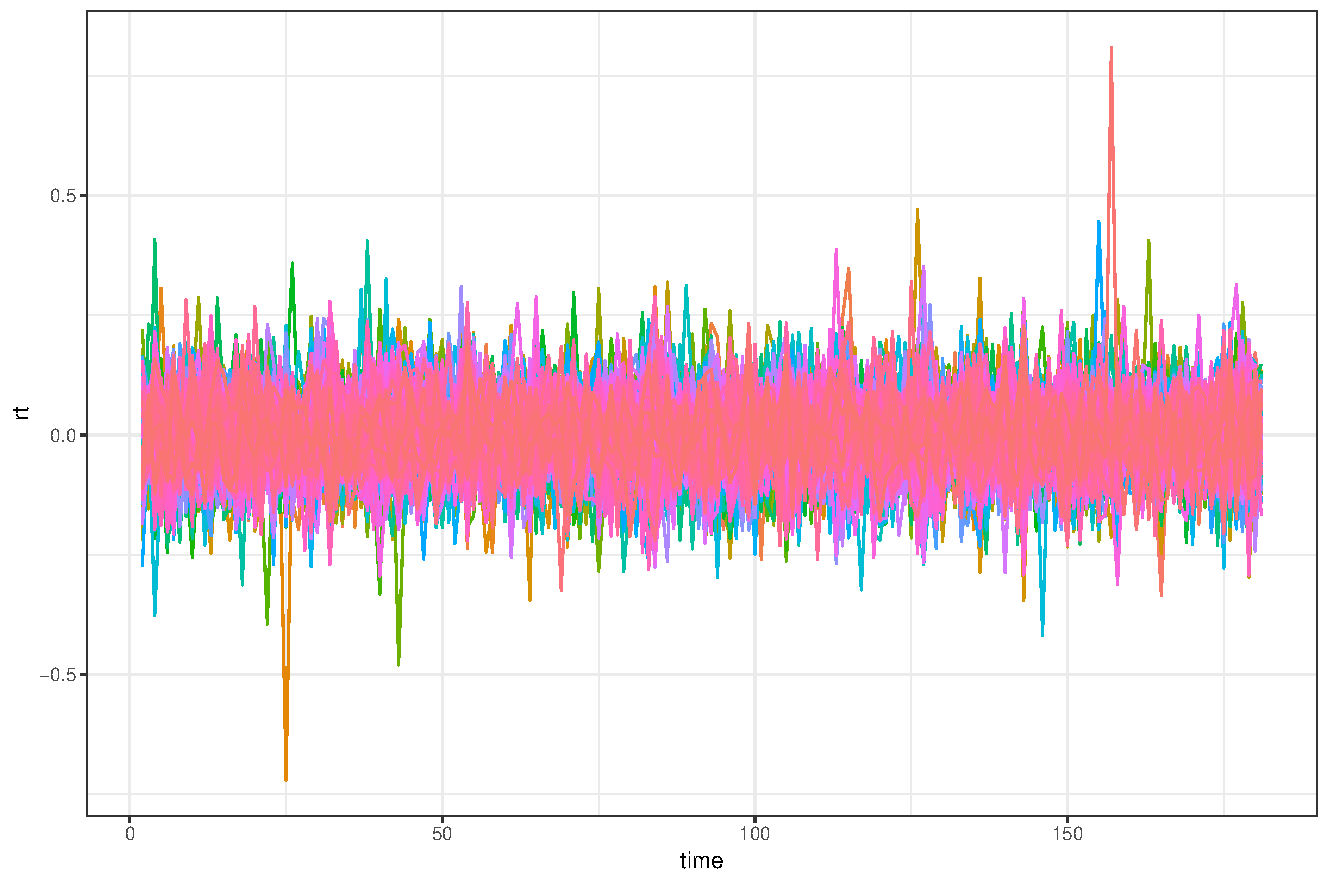
\includegraphics[max size={\textwidth}{0.85\textheight}]{g1_A1_nosv_panel.pdf}
\caption{\cite{gu_empirical_2018}'s Simulation Design}
\end{figure}
\end{frame}

%% OUR DESIGN

\begin{frame}
\frametitle{Proposed Simulation Design}
We propose a design which incorporates:
\begin{itemize}
\item Persistence in regressors
\item Cross sectional correlation in regressors
\item Stochastic volatility in errors
\end{itemize}
\end{frame}

\begin{frame}
\frametitle{Proposed Simulation Design}
Latent factor model with stochastic volatility for excess return, $r_{t+1}$, for $t=1,\dots,T$:

\begin{equation}
r_{i, t+1} = 
g\left(z_{i, t}\right) + \beta_{i,t+1}v_{t+1} + e_{i, t+1}
\end{equation}
\begin{align}
z_{i, t} &=\left(1, x_{t}\right)^{\prime} \otimes c_{i, t}, 
\quad \beta_{i, t}=\left(c_{i 1, t}, c_{i 2, t}, c_{i 3, t}\right) \\ 
e_{i, t+1} &= 
\sigma_{i, t+1} \varepsilon_{i, t+1}; \\
\operatorname{log} (\sigma^2_{i,t+1}) &= 
\omega + \gamma \operatorname{log} (\sigma^2_{t}) + \sigma_{u}u; 
\quad u \sim N(0, 1)
\end{align}

$v_{t+1}$ is a $3\times 1$ vector of errors, $w_{i,t+1},\varepsilon_{i,t+1}$ are scalar error terms.

Parameters tuned s.t. annualized volatility is 20\%.
\end{frame}

\begin{frame}
\frametitle{Simulating Characteristics}

Matrix $C_t$ is an $N\times P_c$ vector of latent factors. 

Build in correlation across time among factors by drawing normal random numbers for each $1\leq i\leq N$ and $1\leq j\leq P_{c}$, according to 

\begin{equation}
\overline{c}_{i j, t} = \rho_{j} \overline{c}_{i j, t-1}+\epsilon_{i j, t} ;
\quad \rho_{j} \sim \mathcal{U} \left( \frac{1}{2},1 \right) 
\end{equation}
\end{frame}

\begin{frame}
\frametitle{Simulating Characteristics}
Then, define the matrix $B$:
\begin{equation}
B:=\Lambda\Lambda' + \frac{1}{10}\mathbb{I}_{n}, \quad
\Lambda_i = (\lambda_{i1},\dots,\lambda_{i4}), \quad
\lambda_{ik}\sim N(0, \lambda_{sd}), \; k=1, \dots, 4
\end{equation}

$B$ is a p.s.d. matrix, serves as a vcov matrix with $\lambda_{sd}$ controlling the \textbf{density} of the matrix. $\lambda_{sd}$ values of 0.01, 0.1 and 1 were used to explore effects of \textbf{cross sectional correlation}.

Simulate characteristics according to

\begin{equation}
\widehat{C}_{t}=L\overline{C}_{t} ; \quad B = LL' 
\end{equation}

where $L$ represents the lower triangle matrix of $B$ using the Cholesky decomposition.
\end{frame}

\begin{frame}
\frametitle{Simulating Characteristics}
Simulate macroeconomic factors according to:

\begin{flalign*}
x_{t} = Ax_{t-1}+u_t; 
\quad A = 
\begin{pmatrix}
.95 & 0 & 0 \\
0 & .95 & 0 \\
0 & 0 & .95
\end{pmatrix} \;
\quad u_t \sim N\left( \mu = (0, 0, 0)' , \Sigma = I_3
\right) 
\end{flalign*}

\end{frame}

\begin{frame}
\frametitle{Simulating Characteristics}

Finally, the "observed" characteristics for each $1\leq i\leq N$ and for $j=1, \dots, P_{c}$ are constructed according to:

\begin{equation}
c_{i j, t} = \frac{2}{n+1} \operatorname{rank}\left(\hat{c}_{i j, t}\right) - 1.
\end{equation}

with the rank transformation normalizing all predictors to be within $[-1, 1]$ 
\end{frame}

\begin{frame}
\frametitle{Simulating Return Series}
We will consider 3 different functions $g(\cdot)$:
\begin{flalign*}
(1)\; & g_1 \left(z_{i, t}\right)=\left(c_{i 1, t}, c_{i 2, t}, c_{i 3, t} \times x_{3,t}'\right) \theta_{0} \\
(2)\; & g_2 \left(z_{i, t}\right)=\left(c_{i 1, t}^{2}, c_{i 1, t} \times c_{i 2, t}, \operatorname{sgn}\left(c_{i 3, t} \times  x_{3,t}'\right)\right) \theta_{0} \\
(3)\; & g_3 \left(z_{i, t}\right) = \left(1[c_{i3,t}>0],c_{i 2, t}^{3}, c_{i 1, t} \times c_{i 2, t}\times 1[c_{i3,t}>0], \text{logit}\left({c}_{i 3, t} \right)\right) \theta_{0}
\end{flalign*}

Tune $\theta^0$ s.t. predictive $R^2$ is 5\% to ensure \textbf{low signal to noise ratio}.

Note that $g_2$ is the most non-linear and \textbf{difficult to approximate}, given the observed characteristics.
\end{frame}

\begin{frame}
\frametitle{Simulating Return Panel}
Each realization results in a panel of:
\begin{itemize}
	\item $N = 200$ stocks
	\item $T = 180$ periods
	\item $P_c = 100$ characteristics
\end{itemize}
A total of 10 realizations were simulated and had models fitted to them.
\end{frame}

\begin{frame}
\frametitle{Simulating Returns Panel}
\begin{figure}
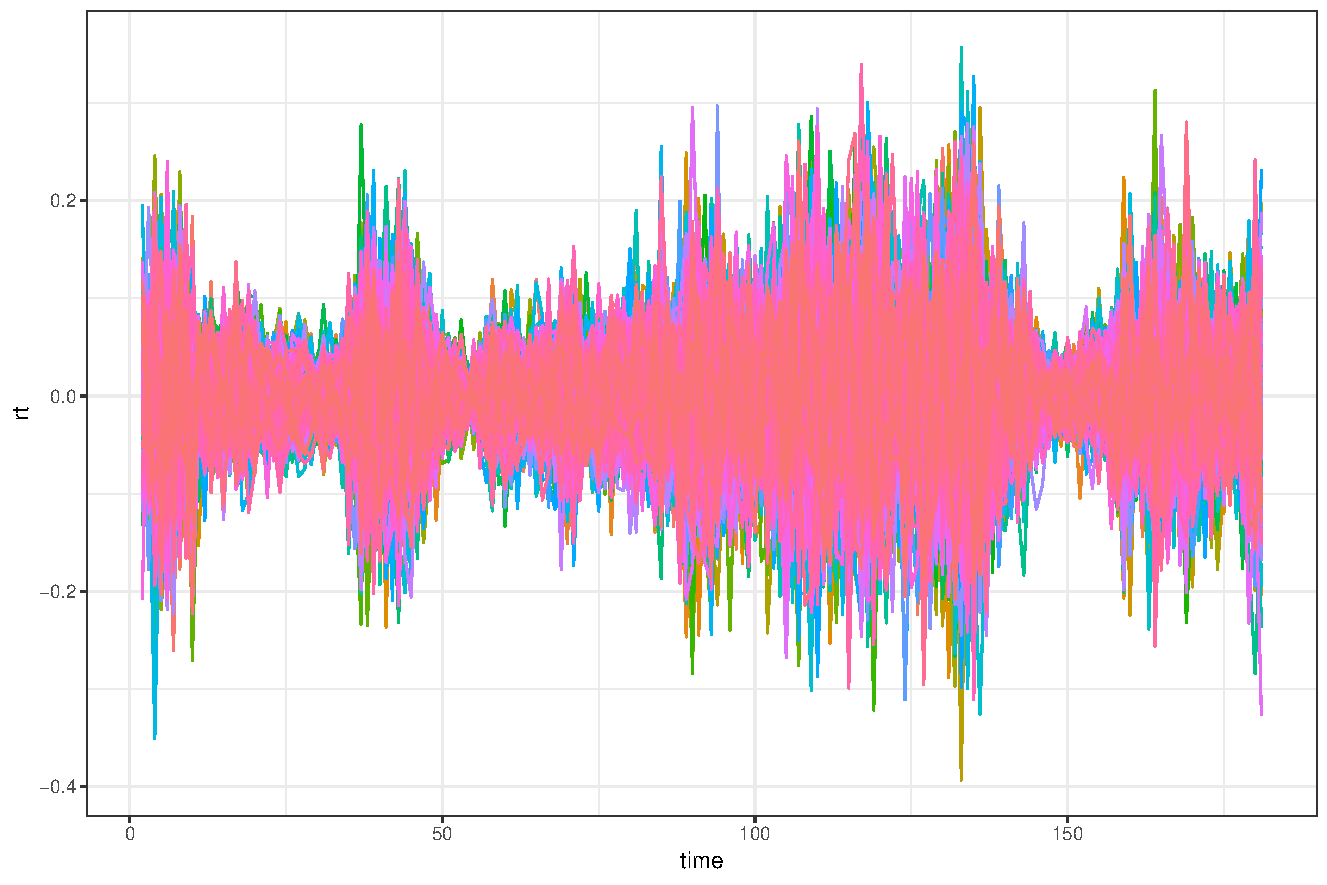
\includegraphics[max size={\textwidth}{0.70\textheight}]{g1_A1_sv_panel.pdf}
\caption{Proposed Simulation Design, 1 Realization}
\end{figure}
\begin{figure}

\end{figure}
\end{frame}

%%%%%%%%%%%%%%%%%%%%%%%%%%%%%%%%%
% SIMULATION STUDY RESULTS

\section{Simulation Study Results}

\begin{frame}
\frametitle{Simulation Results}
Key Results:
\begin{itemize}
\item Minimizing quantile loss is better
\item Elastic Net $>$ Random Forests $>$ Neural Networks $>$ Linear Models
\item Cross sectional correlation \textbf{does not affect prediction performance} by much
\item Elastic net is best for causal analysis, \textbf{even with multicollinearity}
\item Random Forest is better in non-linear settings
\item Neural Networks \textbf{did not outperform}
\item Deeper neural networks seem to do better
\end{itemize}
\end{frame}

\subsection{Prediction Performance}

%% Quantile Loss is better

\begin{frame}
\begin{center}
	\begin{figure}
		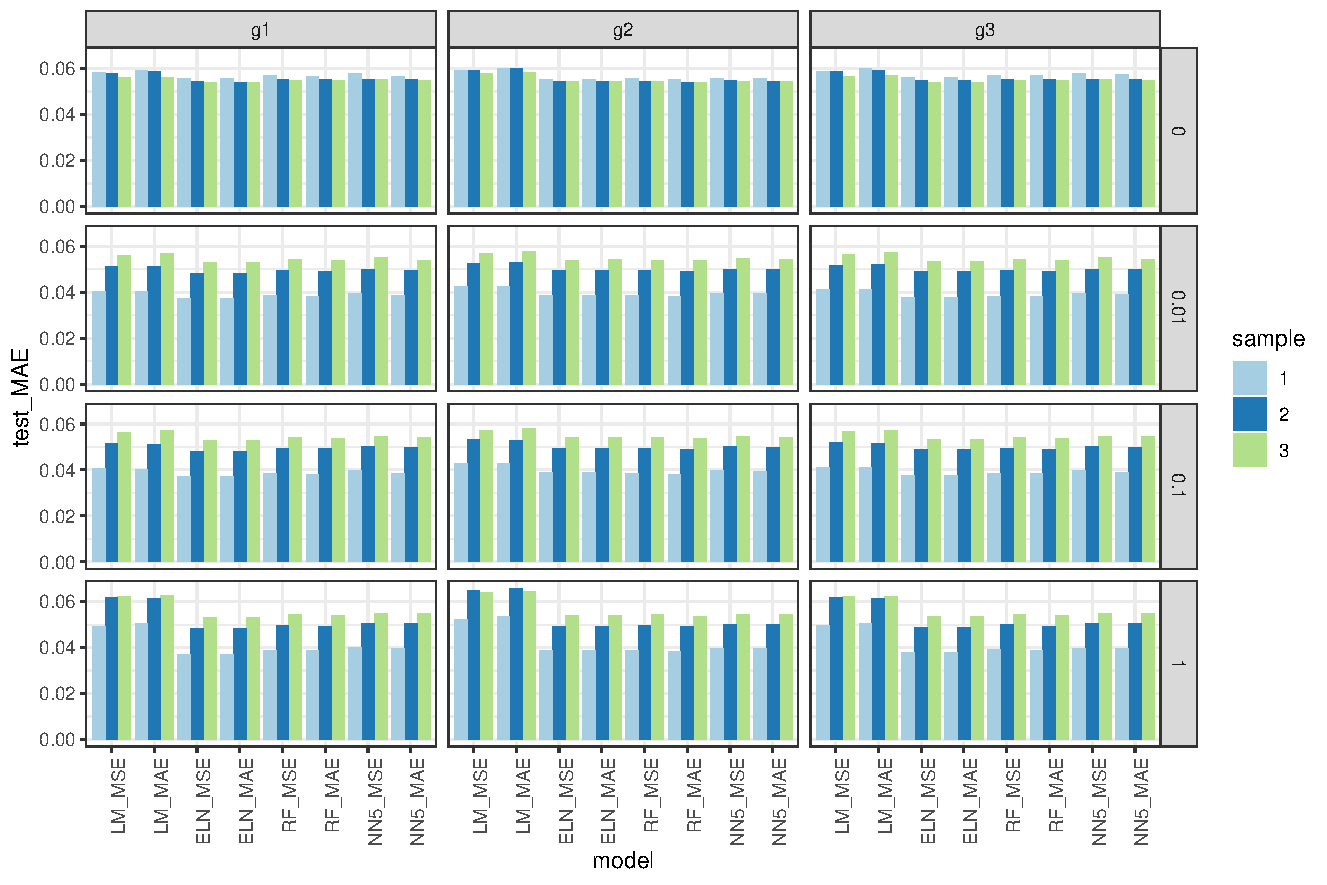
\includegraphics[max size={\textwidth}{0.85\textheight}]{simulation_test_mae_pre_all.pdf}
		\caption{Test MAE across all simulation designs}
	\end{figure}	
\end{center}
\end{frame}

\begin{frame}
\begin{center}
	\begin{figure}
	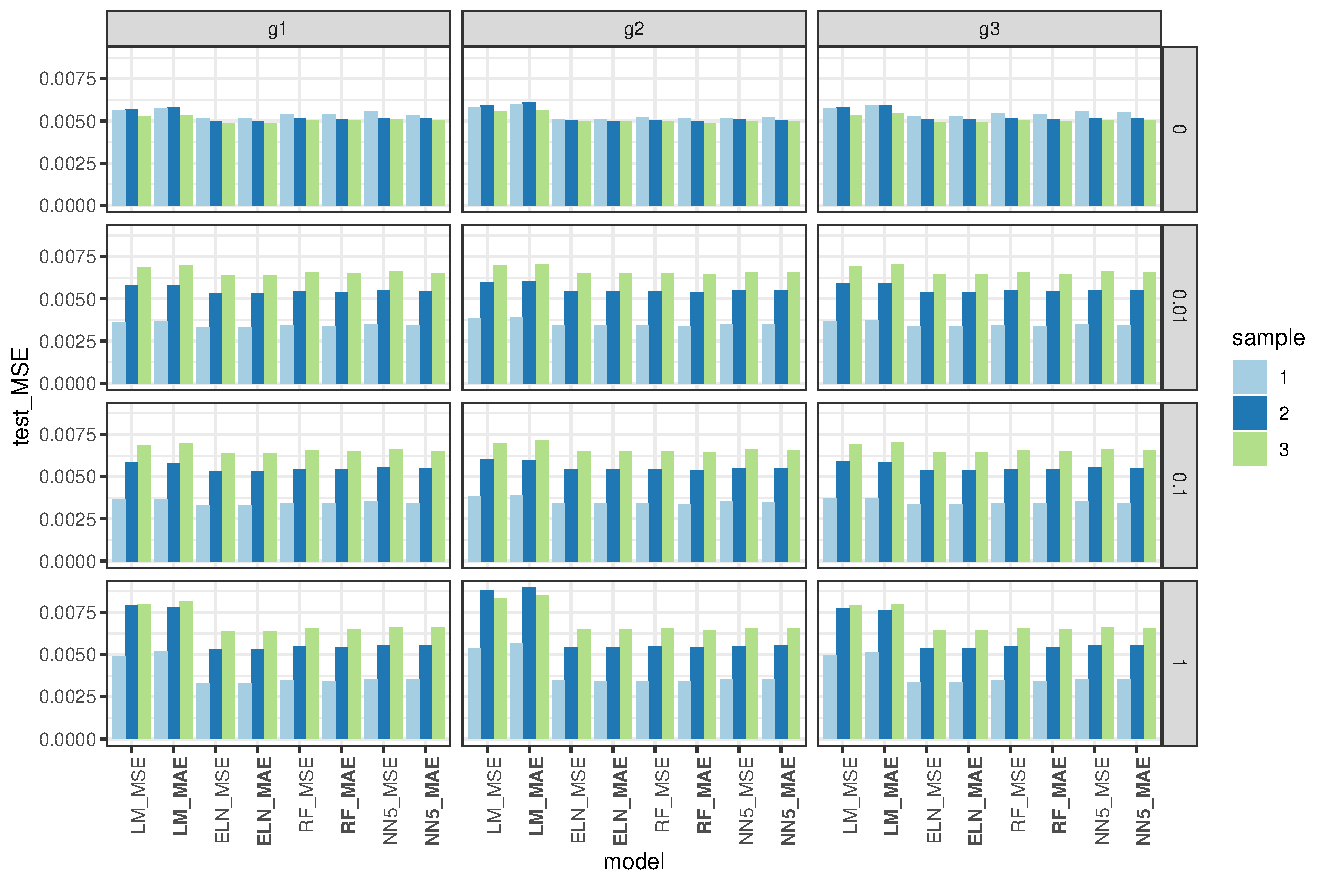
\includegraphics[max size={\textwidth}{0.85\textheight}]{simulation_test_mse_pre_all.pdf}
	\caption{Test MSE across all simulation designs}
	\end{figure}	
\end{center}
\end{frame}

%% More data is worse for SV designs

%% Closer look

\begin{frame}
	\begin{center}
		\begin{figure}
			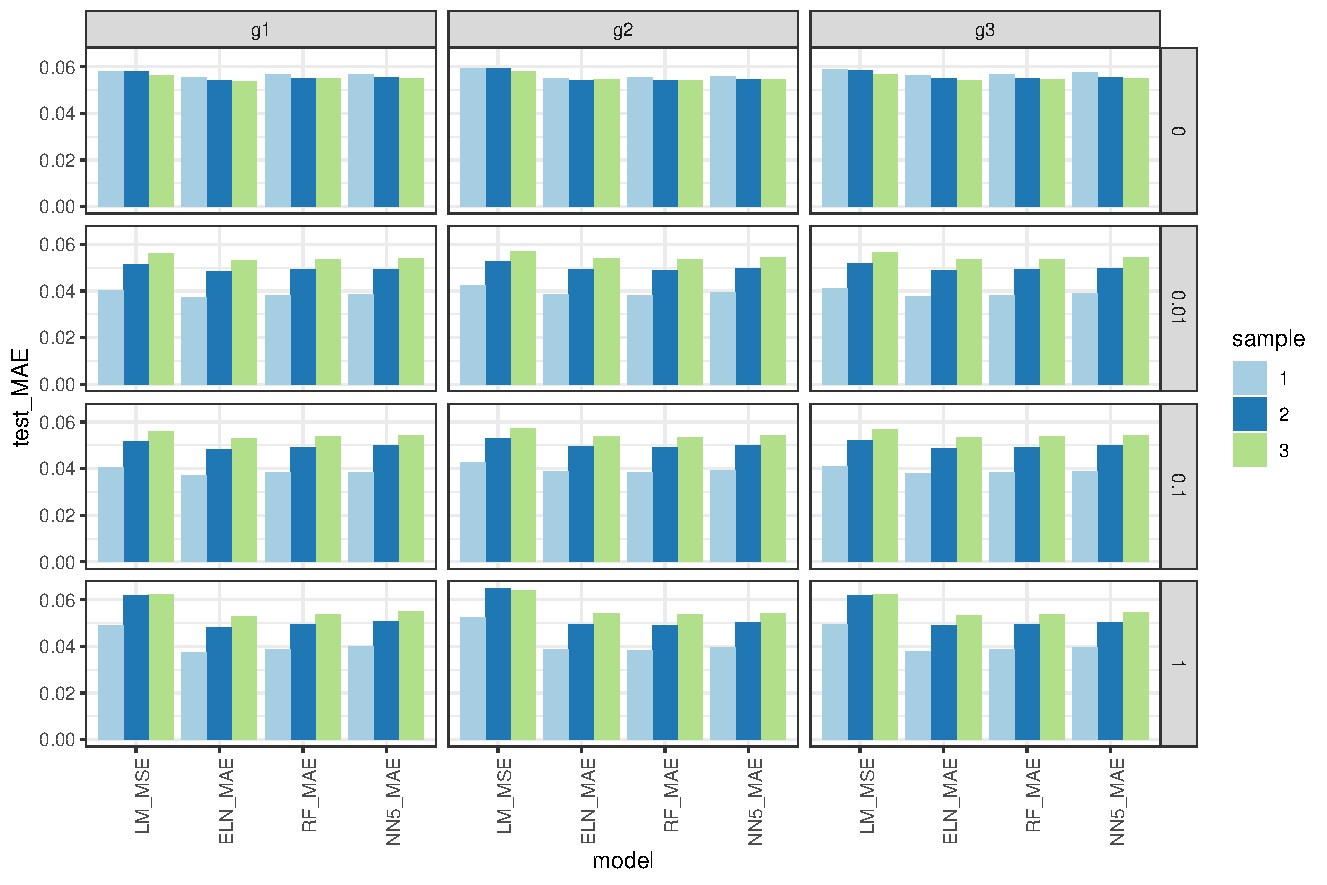
\includegraphics[max size={\textwidth}{0.85\textheight}]{simulation_test_mae_small.pdf}
			\caption{Test MAE across all simulation designs}
		\end{figure}	
	\end{center}
\end{frame}

\begin{frame}
	\begin{center}
		\begin{figure}
			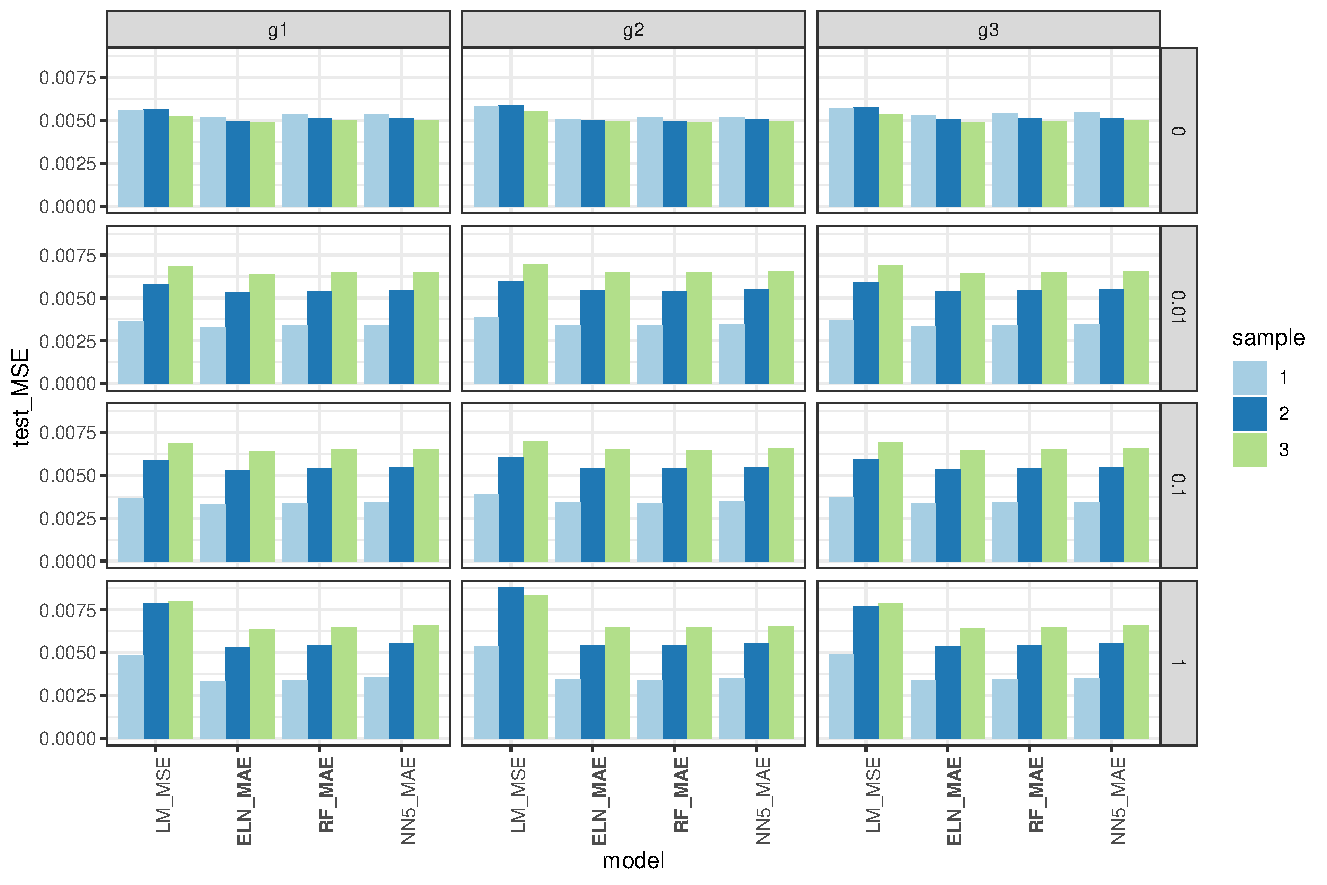
\includegraphics[max size={\textwidth}{0.85\textheight}]{simulation_test_mse_small.pdf}
			\caption{Test MSE across all simulation designs}
		\end{figure}	
	\end{center}
\end{frame}

\begin{frame}
	\begin{center}
		\begin{figure}
			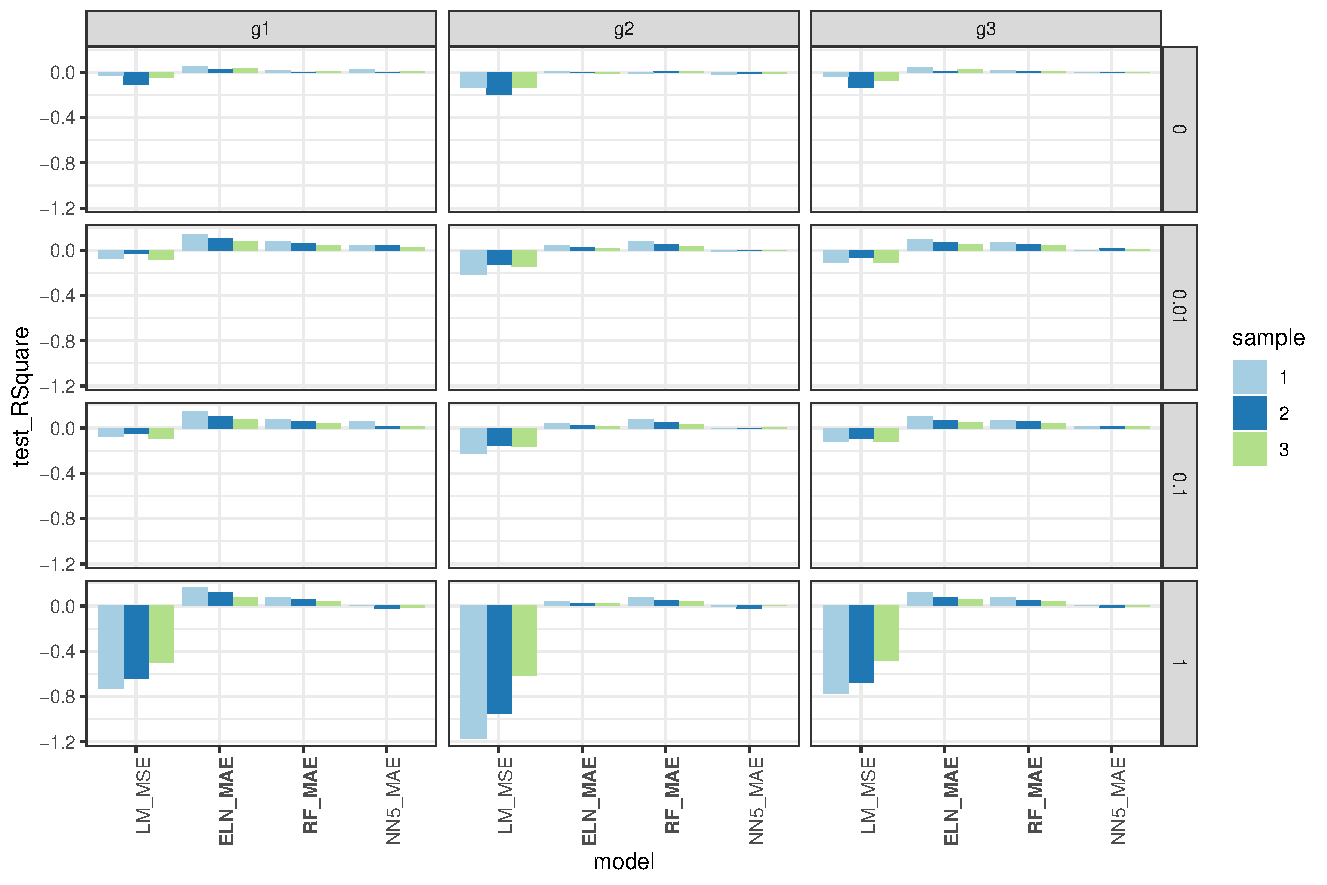
\includegraphics[max size={\textwidth}{0.85\textheight}]{simulation_test_rsquare_small.pdf}
			\caption{Test R Squared Across All Simulation Designs}
		\end{figure}	
	\end{center}
\end{frame}

%% Best Models are penalized Linear and random forests, random forests are only better on g2 specification (most non-linear)

%% Focusing on Neural Networks

%% MAE and MSE are too hard to see the correct trend, so just report R square here. Gets the same point across anyway

\begin{frame}
	\begin{center}
		\begin{figure}
			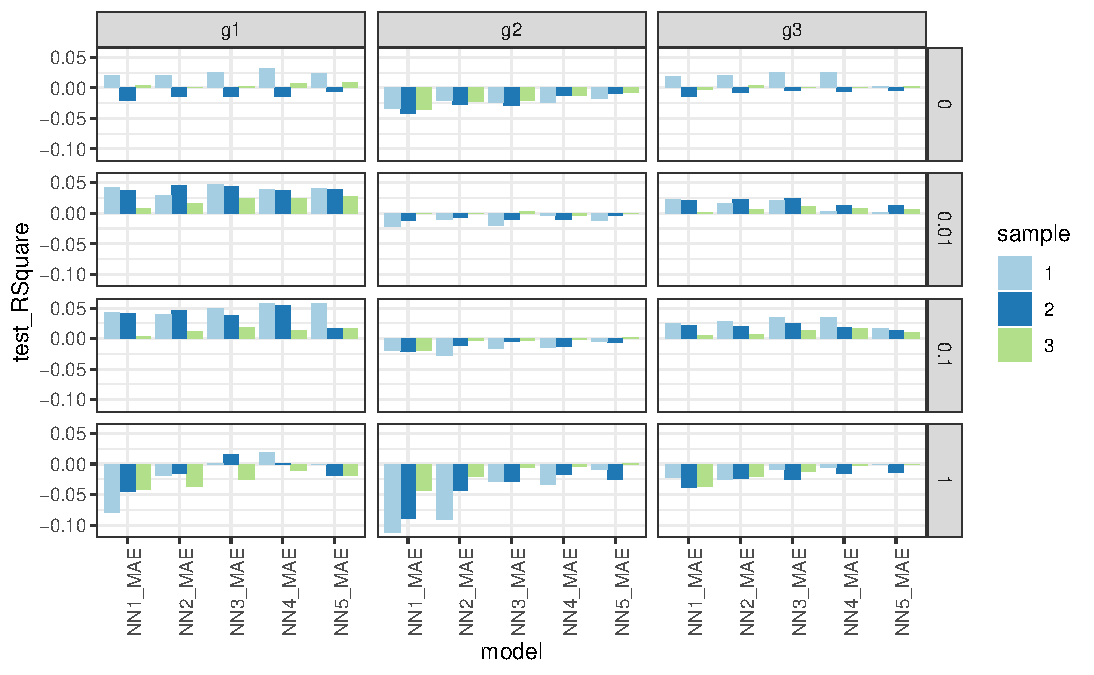
\includegraphics[max size={\textwidth}{0.85\textheight}]{simulation_test_rsquare_small_nn.pdf}
			\caption{Test R Squared Across All Simulation Designs}
		\end{figure}	
	\end{center}
\end{frame}

\subsection{Variable Importance}

\begin{frame}
\begin{center}
	\begin{figure}
	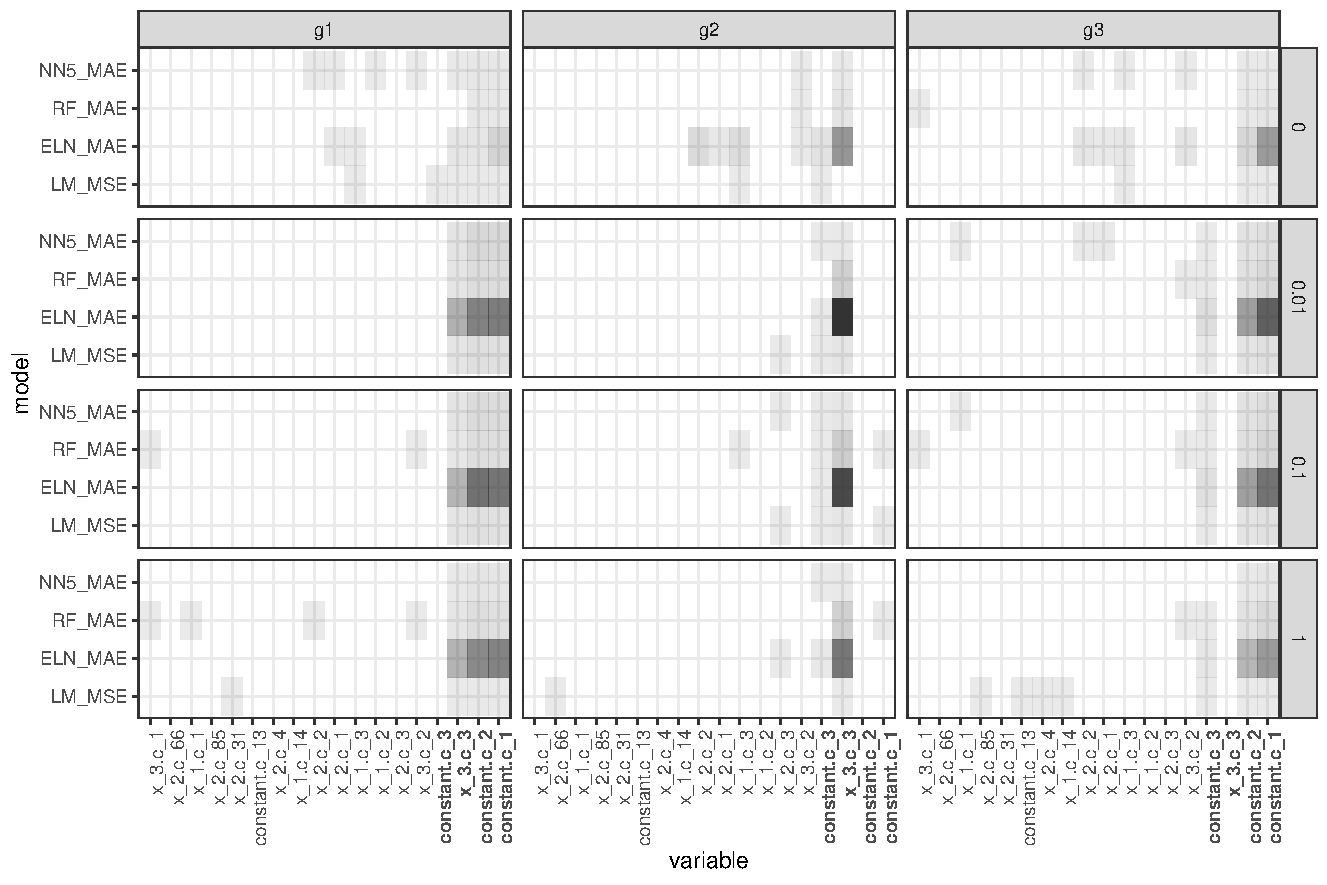
\includegraphics[max size={\textwidth}{0.85\textheight}]{simulation_ave_vi_plot_pre.pdf}
	\caption{Variable Importance Across All simulation Designs}
	\end{figure}
\end{center}
\end{frame}

%% Focus on Neural Networks

\begin{frame}
	\begin{center}
		\begin{figure}
			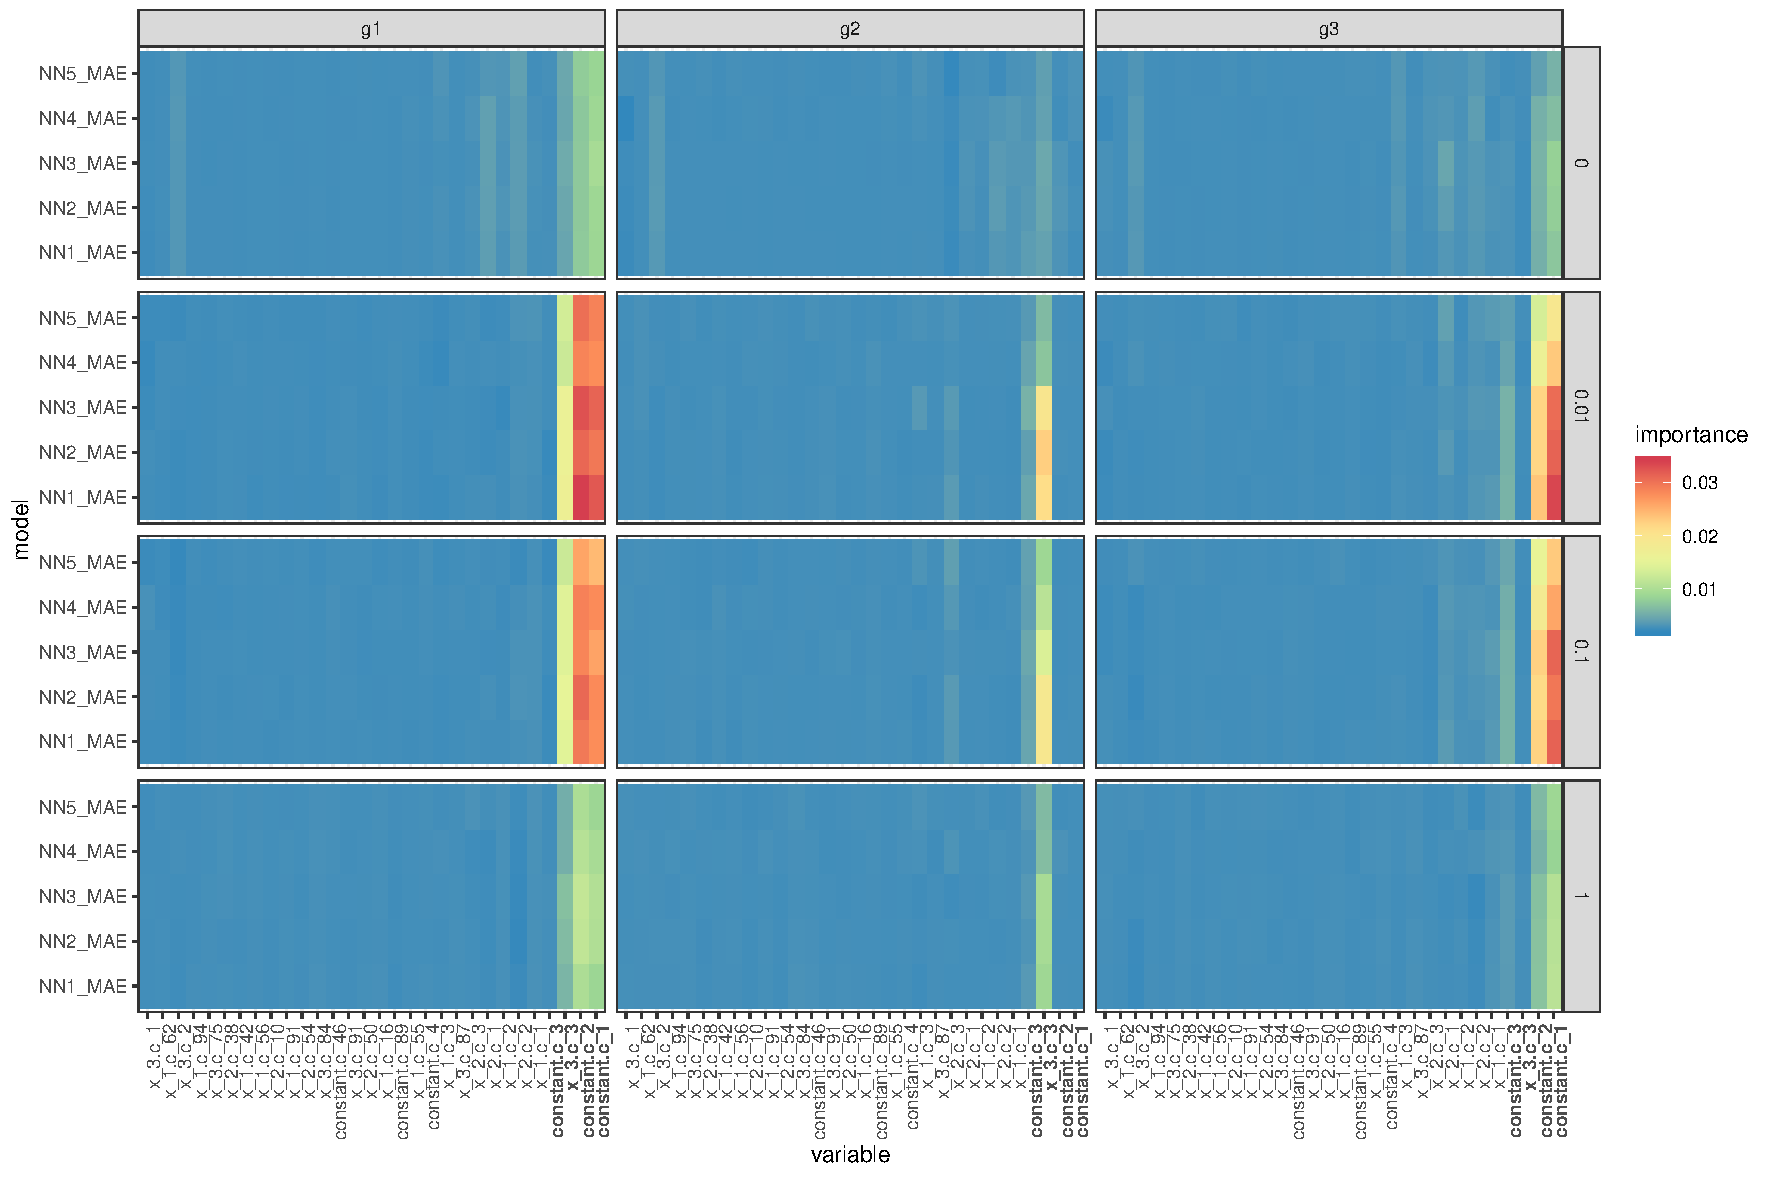
\includegraphics[max size={\textwidth}{0.85\textheight}]{simulation_ave_vi_plot_pre_nn.pdf}
			\caption{Variable Importance Across All simulation Designs, Neural Networks}
		\end{figure}
	\end{center}
\end{frame}

%%%%%%%%%%%%%%%%%%%%%%%%%%%%%%%%%%%%%%%%%%%%%%%%%%%%
\section{Empirical Study}
%%%%%%%%%%%%%%%%%%%%%%%%%%%%%%%%%%%%%%%%%%%%%%%%%%%%

\begin{frame}
\frametitle{Empirical Data}
We now focus on the Empirical Data

Will see the results from the simulation study are \textbf{largely the same}
\end{frame}

\subsection{Data}

\begin{frame}
\frametitle{Data Source}
\cite{gu_empirical_2018}'s dataset of individual factors available from their website:
\begin{itemize}
	\item March 1957 - December 2016
	\item 61 annual factors
	\item 13 quarterly factors
	\item 20 monthly factors
	\item Industry dummy with 74 levels
\end{itemize}
\end{frame}

\begin{frame}
\frametitle{Data Cleaning Procedure}
Reducing dataset size:
\begin{itemize}
	\item Only include NASDAQ stocks
	\item Filter out penny stocks (microcaps)
	\item Keep only instruments with share code of 10, 11 (filtering out REITs, etc)
	\item Convert to a \textbf{quarterly} format
	\item Industry dummy was dropped due to inaccuracy and high dimensionality
\end{itemize}
\end{frame}

\begin{frame}
\frametitle{Data Cleaning Procedure}
Missing Data
\begin{itemize}
	\item Significant increase in data quality and availability after 1993 Q3
	\item Factors with more than 20\% missing data were removed
	\item Remaining missing factors were imputed with cross sectional medians
\end{itemize}
\end{frame}

\begin{frame}
\frametitle{Macroeconomic Factors}
\begin{table}
	\caption{Macroeconomic Factors, (\cite{welch_comprehensive_2008})}
	\begin{center}
		\begin{tabular}{lccc} \hline
			No. & Acronym & Macroeconomic Factor \\ \hline
			1 & macro\_dp & Dividend Price Ratio \\
			2 & macro\_ep & Earnings Price Ratio \\
			3 & macro\_bm & Book to Market Ratio \\
			4 & macro\_ntis & Net Equity Expansion \\
			5 & macro\_tbl & Treasury Bill Rate \\
			6 & macro\_tms & Term Spread \\
			7 & macro\_dfy & Default Spread \\
			8 & macro\_svar & Stock Variance \\ \hline
		\end{tabular}
	\end{center}
\end{table}
\end{frame}

\begin{frame}
\frametitle{Cleaned Dataset}
Baseline set of covariates defined as:
\begin{equation}
	z_{i,t} = (1, x_t)' \otimes c_{i,t}
\end{equation}
where $c_{i,t}$ is a $P_c$ matrix of characteristics for each stock $i$, and $(1, x_t)'$ is a $P_x \times 1$ vector of macroeconomic predictors.

Number of covariates in this baseline set is $61 \times (8 + 1) = 549$. 
\end{frame}

%% CURRENTLY NOT WORKING, FIX ASAP

\begin{frame}
\frametitle{Sample Splitting}
\begin{figure}
	\begin{center}
		\begin{tabular}{|c|p{0.60cm}p{0.60cm}p{0.40cm}p{0.40cm}p{0.40cm}p{0.40cm}p{0.40cm}p{0.40cm}p{0.40cm}p{0.40cm}p{0.40cm}p{0.40cm}p{0.40cm}p{0.40cm}p{0.40cm}p{0.40cm}|}
			\hline
			Set &&&&&&&&&&&&&&&& \\
			\hline
			%%%%%%%%
			3 & \cellcolor{cyan} & \cellcolor{cyan} & \cellcolor{cyan} & \cellcolor{cyan} & \cellcolor{cyan} & \cellcolor{cyan} & \cellcolor{cyan} & \cellcolor{cyan} &
			\cellcolor{pink} & \cellcolor{pink} & \cellcolor{pink} & \cellcolor{pink} & \cellcolor{pink} & \cellcolor{pink} & \cellcolor{pink} & \cellcolor{olive} \\
			%%%%%%%%
			2 & \cellcolor{cyan} & \cellcolor{cyan} & \cellcolor{cyan} & \cellcolor{cyan} & \cellcolor{cyan} & \cellcolor{cyan} & \cellcolor{cyan} &
			\cellcolor{pink} & \cellcolor{pink} & \cellcolor{pink} & \cellcolor{pink} & \cellcolor{pink} & \cellcolor{pink} & \cellcolor{pink} & 	
			\cellcolor{olive} & NA \\
			%%%%%%%%
			1 & \cellcolor{cyan} & \cellcolor{cyan} & \cellcolor{cyan} & \cellcolor{cyan} & \cellcolor{cyan} & \cellcolor{cyan} &
			\cellcolor{pink} & \cellcolor{pink} & \cellcolor{pink} & \cellcolor{pink} & \cellcolor{pink} & \cellcolor{pink} & \cellcolor{pink} & \cellcolor{olive} & NA & NA \\
			\hline
			Time & 93Q3 & 93Q4 & 94 & 95 & 96 & ... & 06 & 07 & 08 & ... & 11 & 12 & 13 & 14 & 15 & 16 \\
			\hline
		\end{tabular}
		\medskip
		\begin{tabular}{|c|p{0.60cm}|}
			\hline
			Training & \cellcolor{cyan} \\
			\hline
			Validation & \cellcolor{pink} \\
			\hline
			Test & \cellcolor{olive} \\
			\hline
		\end{tabular}
	\end{center}
	\caption{Empirical Data Sample Splitting Procedure}
	\label{emp_sample_split_diag}
\end{figure}
\end{frame}

\subsection{Empirical Data Results}

\begin{frame}
\frametitle{Overview}

Results \textbf{largely the same} as the simulation study.

Key results:
\begin{itemize}
	\item Minimizing quantile loss is better
	\item Elastic Net $>$ Random Forests $>$ Neural Networks $>$ Linear Models
	\item Elastic Net and Random Forests tend to agree on same subset of predictors
	\item Neural Networks \textbf{did not outperform}
	\item Neural Networks start to fail
\end{itemize}

Many of these results \textbf{contradict} \cite{gu_empirical_2018}'s findings.

\end{frame}

%%%%%%%%%%%%%%%%%%%%%%%%%%%%%%%%%%%%%%%%%%%%%%%%%%%%%%%%%%%%

\subsubsection{Prediction Accuracy}

%% PREDICTION ACCURACY

%% Prove that quantile loss is better first

\begin{frame}
\begin{figure}
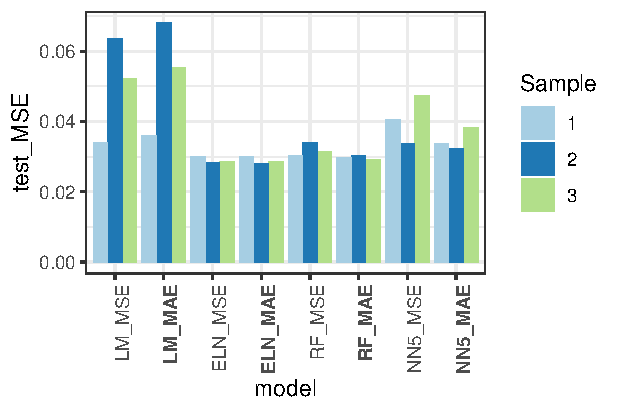
\includegraphics[max size={\textwidth}{0.85\textheight}]{empirical_test_mse_pre_all.pdf}
\caption{Empirical Data Test MSE}
\end{figure}
\end{frame}

\begin{frame}
\begin{figure}
	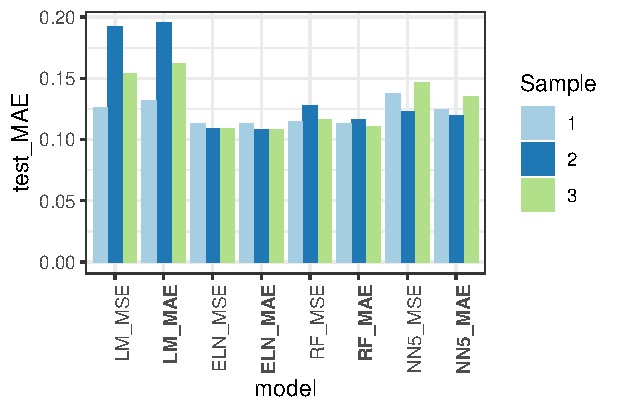
\includegraphics[max size={\textwidth}{0.85\textheight}]{empirical_test_mae_pre_all.pdf}
	\caption{Empirical Data Test MAE}
\end{figure}
\end{frame}

\begin{frame}
	\begin{figure}
		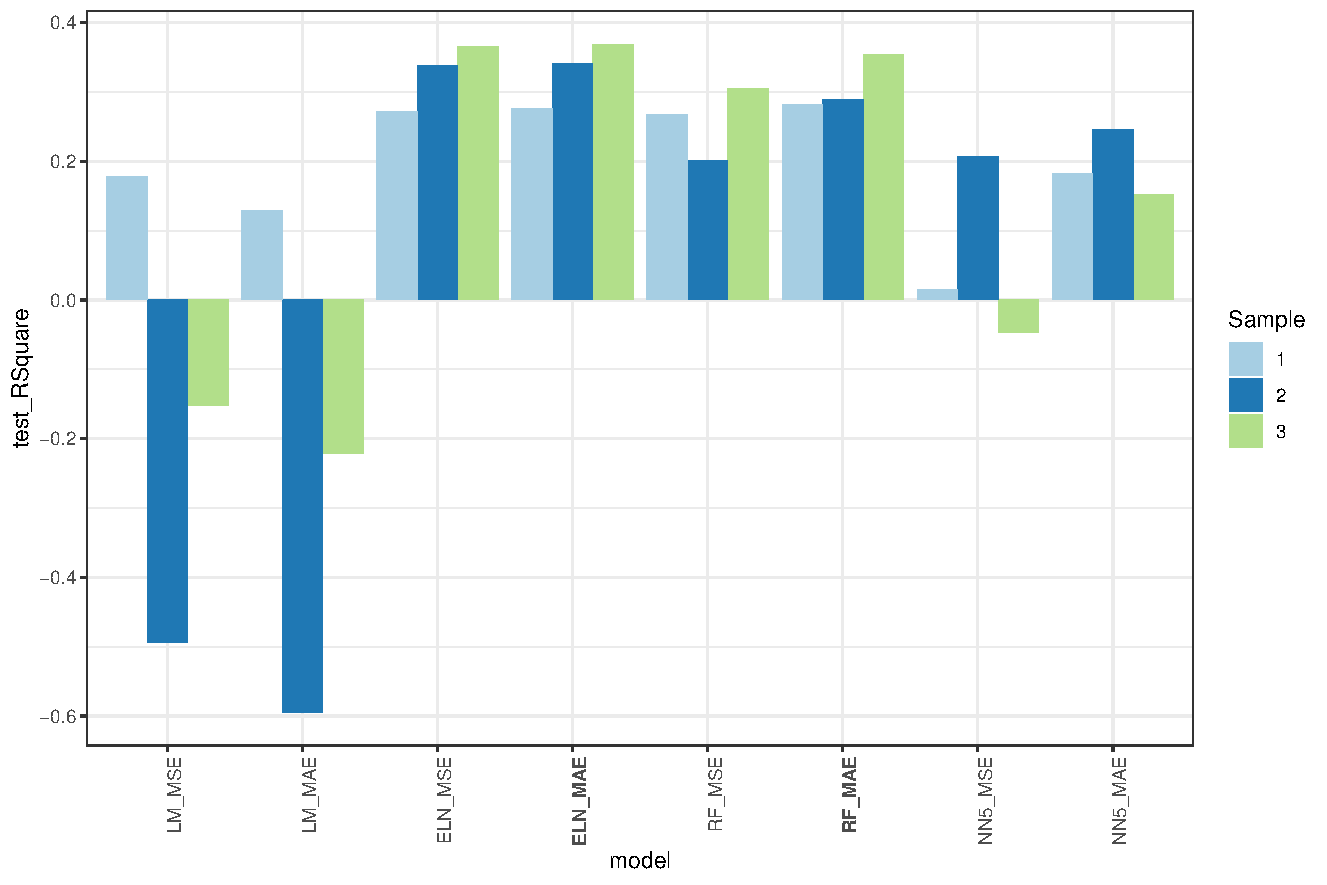
\includegraphics[max size={\textwidth}{0.85\textheight}]{empirical_test_rsquare_pre_all.pdf}
		\caption{Empirical Data Test R Squared}
	\end{figure}
\end{frame}

\begin{frame}
\frametitle{Prediction Performance Results}

Elastic Net $>$ Random Forests $>$ Neural Networks $>$ Linear Models

More data did not seem adversely affect prediction performance - data considered may have had less shocks than simulated datasets

Neural Networks are much more unstable on empirical data, especially when using MSE as a loss function

Weak evidence that deeper neural networks are better
\end{frame}

%% Focusing on Neural Networks

\begin{frame}
	\begin{figure}
		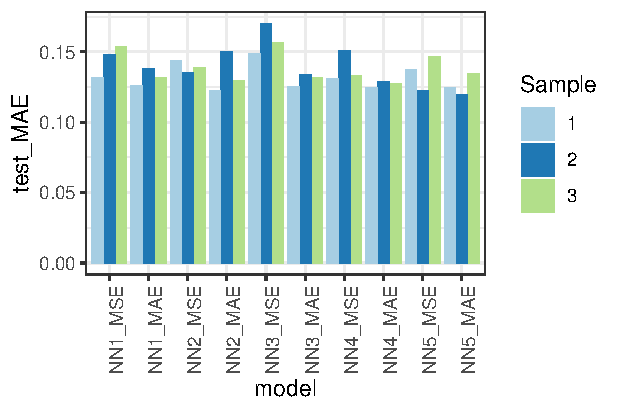
\includegraphics[max size={\textwidth}{0.85\textheight}]{empirical_test_mae_pre_nn.pdf}
		\caption{Empirical Data Test MAE for Neural Networks}
	\end{figure}
\end{frame}

\begin{frame}
	\begin{figure}
		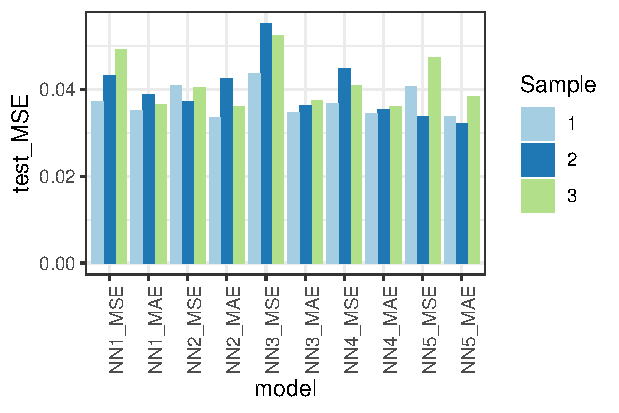
\includegraphics[max size={\textwidth}{0.85\textheight}]{empirical_test_mse_pre_nn.pdf}
		\caption{Empirical Data Test MSE for Neural Networks}
	\end{figure}
\end{frame}

\begin{frame}
	\begin{figure}
		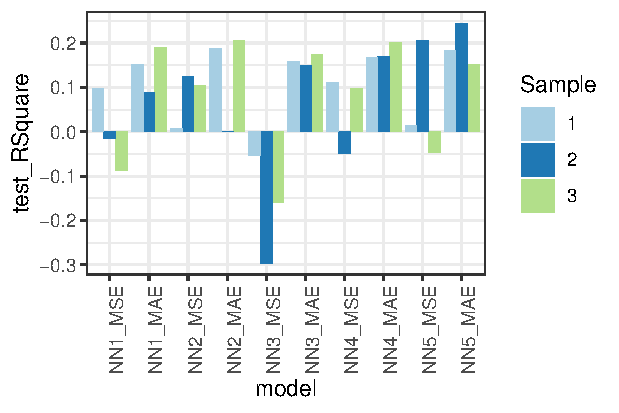
\includegraphics[max size={\textwidth}{0.85\textheight}]{empirical_test_rsquare_pre_nn.pdf}
		\caption{Empirical Data Test R Squared for Neural Networks}
	\end{figure}
\end{frame}

%%%%%%%%%%%%%%%%%%%%%%%%%%%%%%%%%%%%%%%%%%%%%%%%%%%%%%%%%%%
%% VARIABLE IMPORTANCE

\subsubsection{Variable Importance}

\begin{frame}
\frametitle{Variable Importance Results}
Difficult to compare with simulation results, as underlying DGP is unknown

However, similar trends can be observed:
\begin{itemize}
	\item Elastic Net and Random Forests agree on same subset
	\item Random Forest struggle to discern between factors
	\item Neural Networks results are completely different
\end{itemize}
\end{frame}

%% INDIVIDUAL VARIABLE IMPORTANCE

\begin{frame}
	\begin{figure}
	\begin{center}
		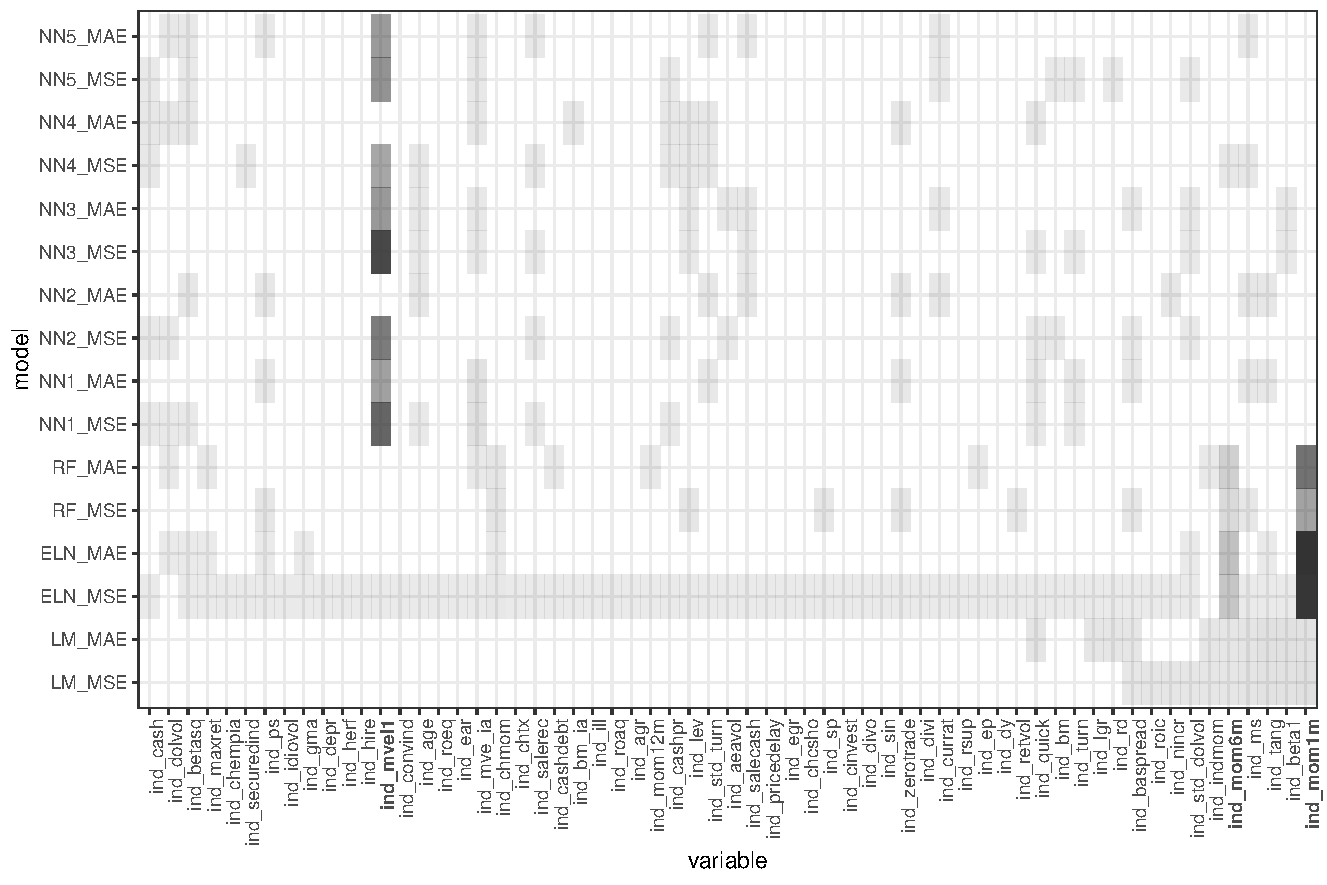
\includegraphics[max size={\textwidth}{0.85\textheight}]{empirical_sample_all_vi_ind.pdf}
		\caption{Empirical Individual Factor Importance, averaged over all samples}
	\end{center}
\end{figure}
\end{frame}

%% MACROECONOMIC

\begin{frame}
	\begin{figure}
	\begin{center}
		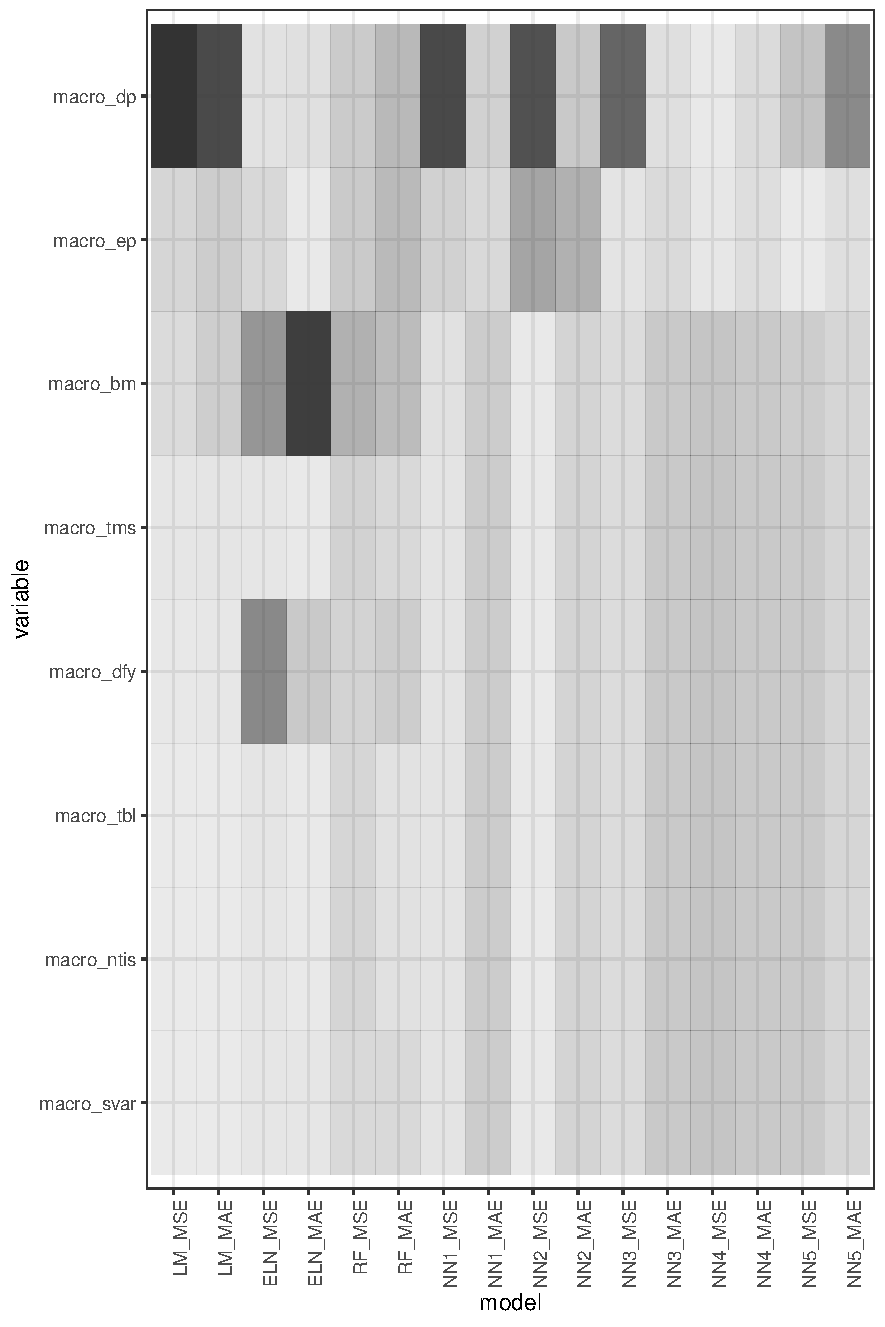
\includegraphics[max size={\textwidth}{0.85\textheight}]{empirical_sample_all_vi_macro.pdf}
		\caption{Empirical Macroeconomic Factor Importance, averaged over all samples}
	\end{center}
\end{figure}
\end{frame}

\begin{frame}
	\begin{figure}
		\begin{center}
			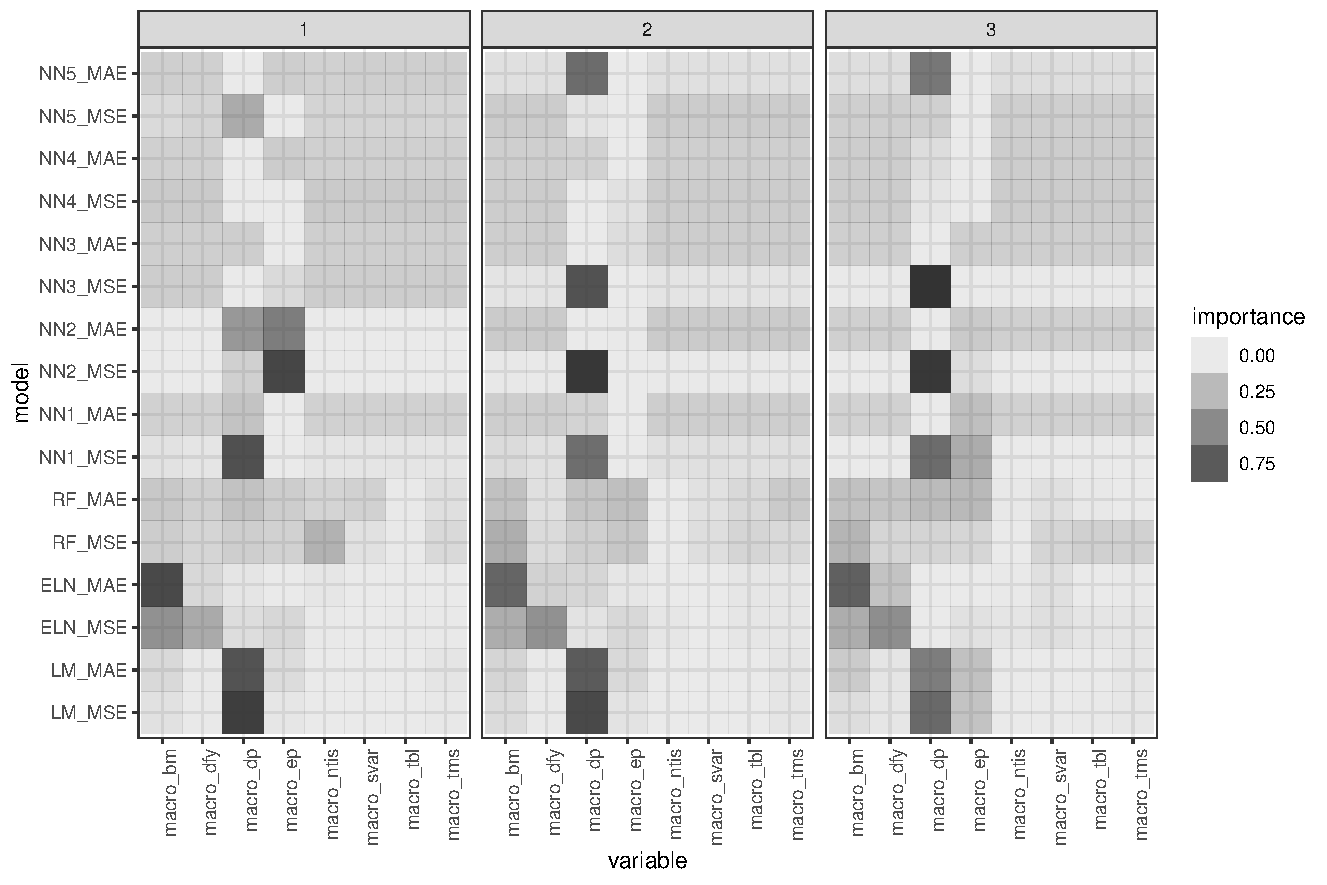
\includegraphics[max size={\textwidth}{0.85\textheight}]{empirical_sample_all_vi_macro_facet.pdf}
			\caption{Empirical Macroeconomic Factor Importance, averaged over all samples}
		\end{center}
	\end{figure}
\end{frame}

\begin{frame}
\frametitle{Variable Importance}
Elastic Net and Random Forests:
\begin{itemize}
\item 1 and 6 month momentum factors
\item Book-to-market Ratio and Default Spread
\end{itemize}
Factors in Neural Networks (\textbf{inconsistent}):
\begin{itemize}
\item Individual Market Value 
\item Dividend-price Ratio and Earnings-price Ratio 
\end{itemize}
\end{frame}

%%%%%%%%%%%%%%%%%%%%%%%%%%%%%%%%%%%%%%%%%%%%%%%%%%%%
\section{Conclusion}
%%%%%%%%%%%%%%%%%%%%%%%%%%%%%%%%%%%%%%%%%%%%%%%%%%%%
\begin{frame}
\frametitle{Conclusion}

Machine learning offers tools to improve stock return prediction and identification of true underlying regressors. 

Elastic Net and Random Forests are the best performing models.

Feed-forward neural networks considered did not outperform.

Elastic Net and Random Forests agree and correctly identify causal regressors. Neural networks only agree in simulated contexts. 

Cross sectional correlation does not affect prediction performance of machine learning by much.

Minimizing quantile loss yields better prediction performance.
\end{frame}

\begin{frame}
\frametitle{Contribution to Literature}
Overall findings differ from sparse literature on similar topics.

Results are consistent across simulated data and empirical data, suggesting a robust set of results.

Overall, results are promising, especially for Elastic Net.
\end{frame}

\begin{frame}
\frametitle{Source Code}
Source code is fully available, along with instructions on how to build datasets:

\url{https://github.com/Meron35/Evaluation-of-Machine-Learning-in-Asset-Pricing}
\end{frame}

%%%%%%%%%%%%%%%%%%%%%%%%%%%%%%%%%%%%%%%%%%%%%%%%%%%%
\section{References}
%%%%%%%%%%%%%%%%%%%%%%%%%%%%%%%%%%%%%%%%%%%%%%%%%%%%
%This is just here to get the citations working throughout the presentation, skip over this when presenting
\begin{frame}
\frametitle{References}
\bibliographystyle{jfe}
\bibliography{Bibliography}
\end{frame}

%%%%%%%%%%%%%%%%%%%%%%%%%%%%%%%%%%%%%%%%%%%%%%%%%%%%
\section{Questions and Answers}
%%%%%%%%%%%%%%%%%%%%%%%%%%%%%%%%%%%%%%%%%%%%%%%%%%%%

\begin{frame}
\begin{center}
\huge Questions and Answers
\end{center}
\end{frame}

\end{document}
